\section{Software requirements specification}\label{sec:srs}

\subsection{Problem domain and purpose of our system}\label{ssec:intro}
As mentioned earlier sleep deprivation is a prevalent problem that society faces.
When constructing the application we wanted it to be accessible to the general public as it was identified earlier that sleep deprivation has the potential to affect everyone.
It was identified that the main functionality of our system would be to aid users to track and compare their sleep through the Neuromind headset.

\subsection{Stakeholders involved and the elicitation process:}\label{ssec:stakeholders}
In order to elicit requirements, a questionnaire was constructed. Majority of the stakeholders involved were flight attendants from United Airlines.
In order to get a more diverse range of views to accomodate for diversity, an interview was conducted on a university student with a part time job.
Responses from participants validated our specific problem by justification both in the questionnaire and in the interviews.
We also constructed new requirements from group meetings through the agile process as group members working with specific requirements
identified that requirements could be refined to accomodate for a broader usage.

\subsection{How conflicts between requirements were managed:}\label{ssec:conflicts}
Throughout the course of the project, requirements were refined when group
meetings were conducted and observations by the group were made.
In particular, our team noticed that in order for the system to successfully calculate sleep cycle data,
it had to be extracted from the data calculated by the headset.

Another major requirement that was refined was the client interface.
This initially did not have any sub-requirements, but later sub-requirements had to be added in order for the stakeholder to be able to view processed data.
Without continuous communications between group members and stakeholder contact these optimisations would not have been possible.

Furthermore, towards the end of our project the client requirement remained, but another functional
requirement that we wanted to integrate into our software was the Graphical User Interface (GUI).
It had been expressed in the questionnaire that a graph to view sleep cycle data would be desirable for the end user.
Just having a Graphical user interface independent of the other functionalities would segment our system,
so as a group we devised to incorporate the GUI into our framework to ensure that it would be easier for
the user to interact with the system whilst maintaining a cohesive system.

\subsection{UseCase Diagram:}\label{ssec:UCD}
\begin{figure}[H]
  \centering
  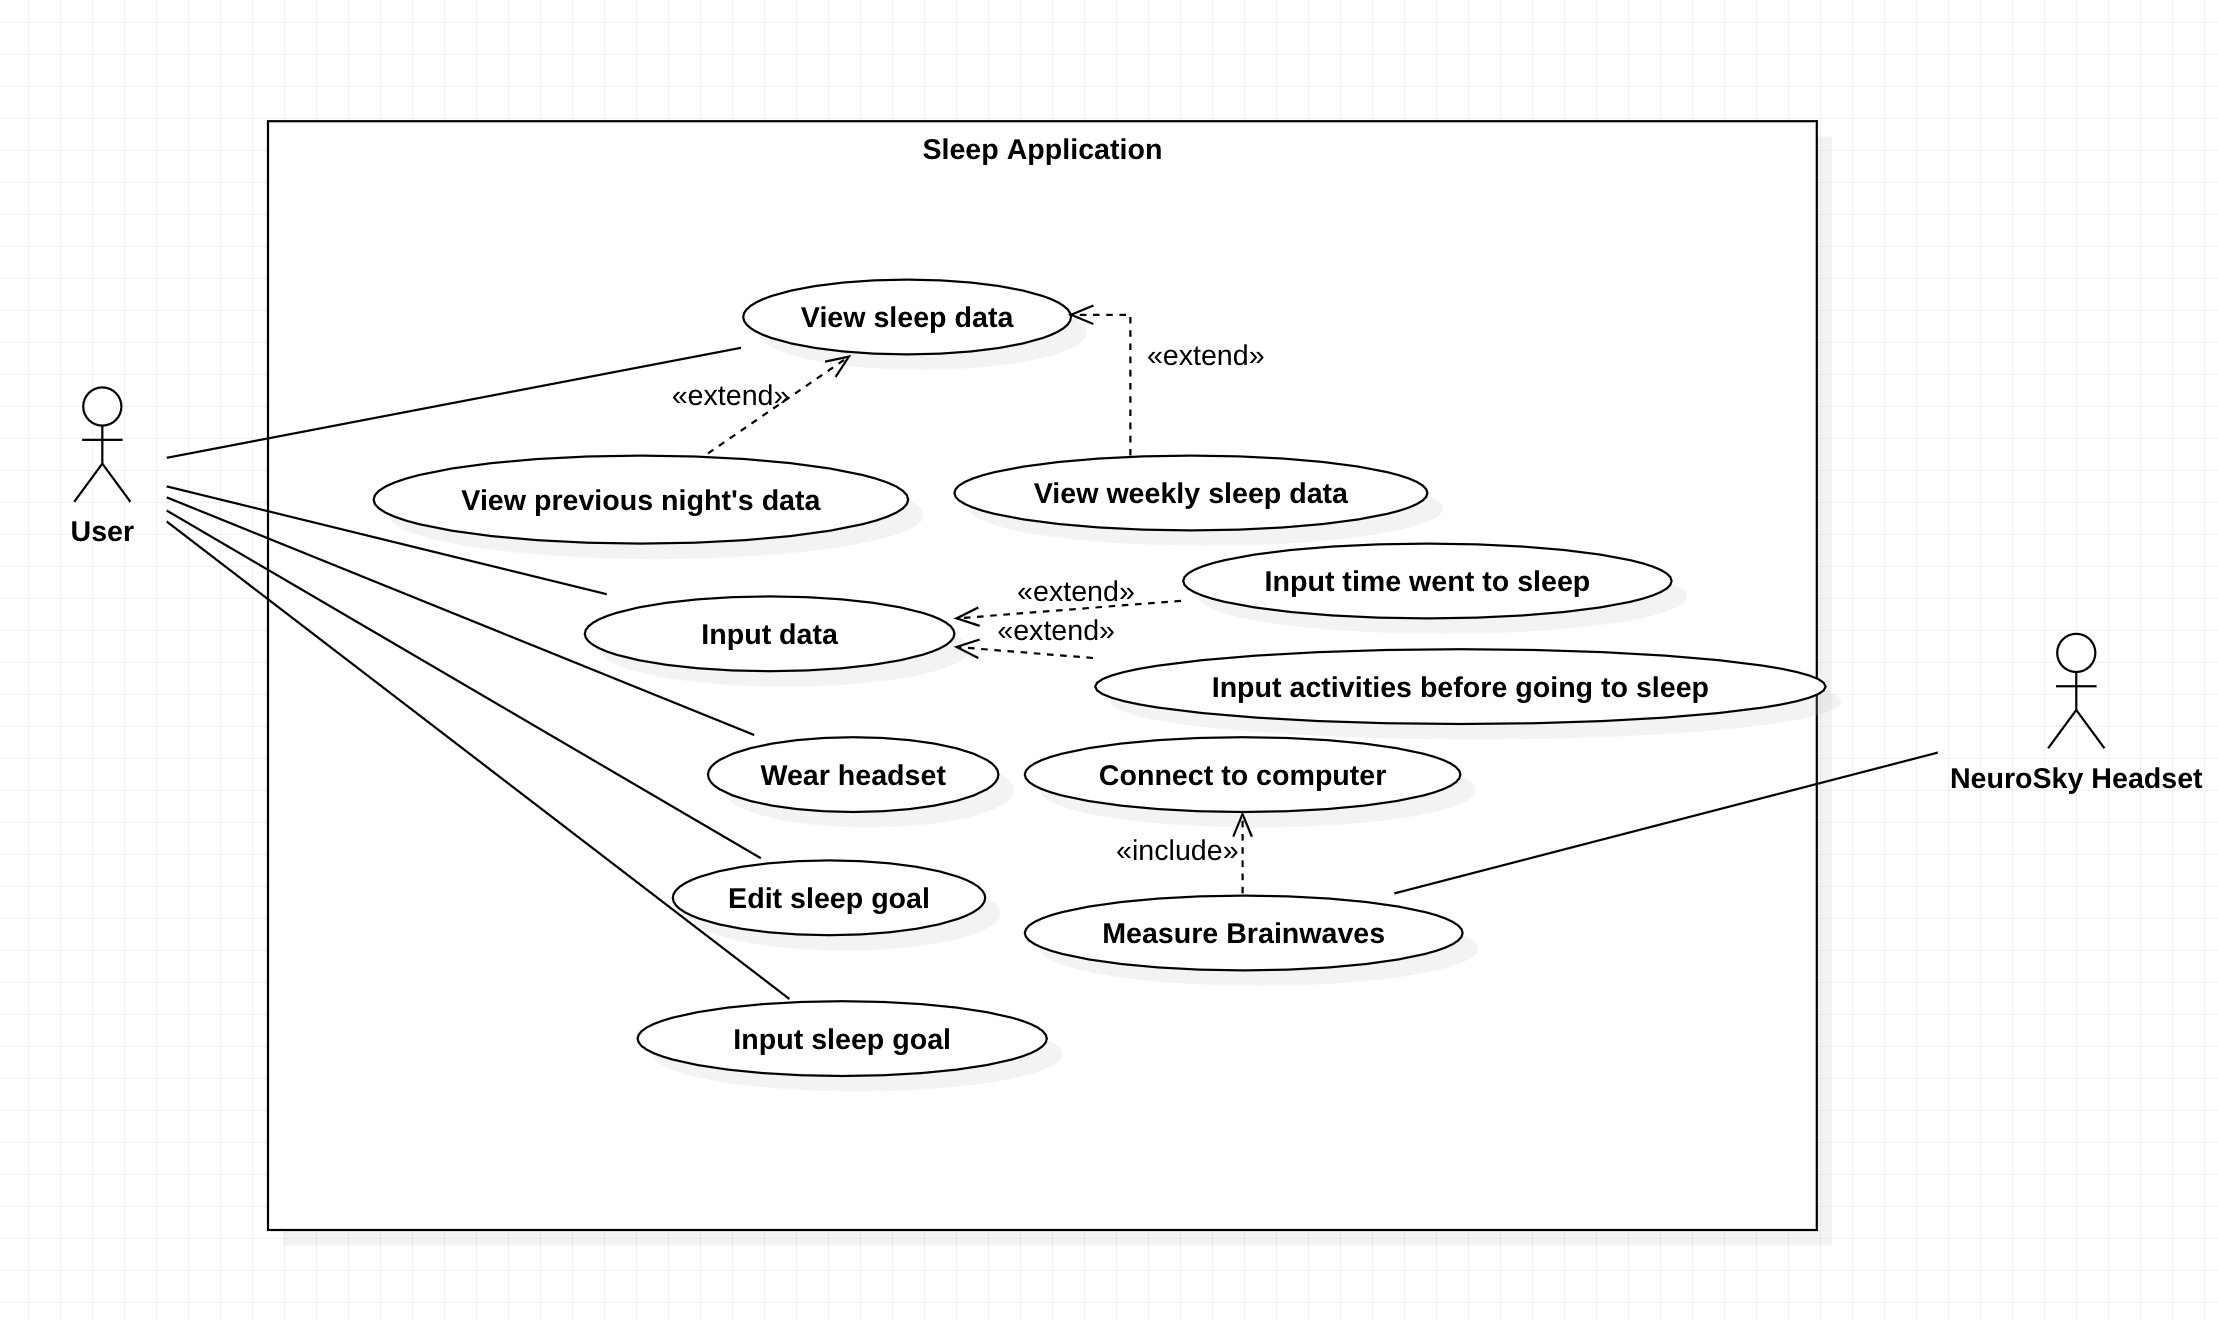
\includegraphics[width=1\textwidth]{UseCaseDiagram}
  \caption{Use Case Diagram}\label{img:use-case-diagram}
\end{figure}
Semantics:
The headset is the external hardware which the user has to wear in order to get a recording.
Once the user is wearing the headset, it can connect to the computer and then measure the user’s brainwaves.
The user is the general audience who will interact with our system.
The user can view sleep data they have inputted into the system using the headset.
They can view either their previous night’s data or last weeks data.
They can also set personal sleep goals which will allow them to then manage their goals that will be saved in the system.
They can also input the time they have previously went to sleep on nights they did not wear the headset.

\subsection{Scenarios:}\label{ssec:scenar}
\subsubsection{Scenario 1:}\label{ssec:scenar1}
Scenario 1:
Actor: User of the system
Goal: Measuring sleep data
Pre conditions:
  1. The user has neurosky headset
  2. The user has thinkgear socket connector installed on their laptop
  3. The user has our application installed.
\begin{figure}[H]
  \centering
  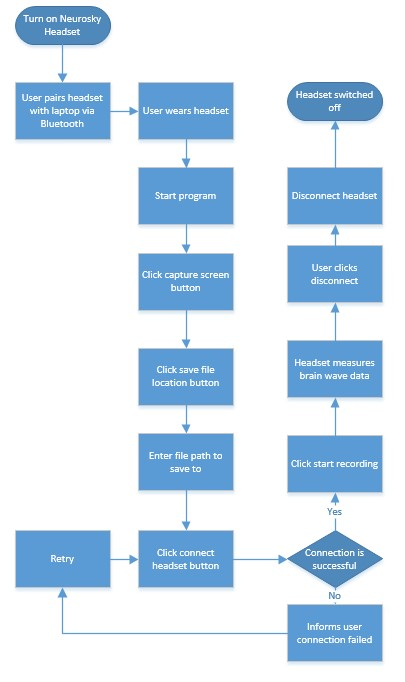
\includegraphics[width=0.5\textwidth]{UseCaseScenario1}
  \caption{Scenario 1}\label{img:usecasescenario1}
\end{figure}

\subsubsection{Scenario 2:}\label{ssec:scenar2}
Scenario 2:
Actor: The user of the system
Goal: View line graph of  brain activity throughout the time the headset was worn.
Preconditions:
The user has the application installed.
Scenario 1 has been completed at least once.
The user has already opened the application.
\begin{figure}[H]
  \centering
  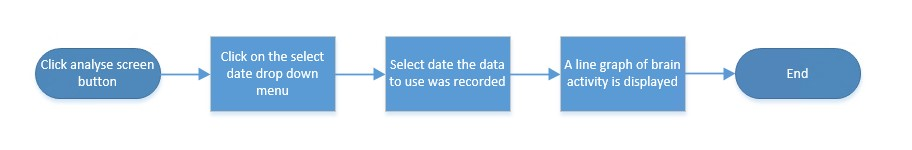
\includegraphics[width=1\textwidth]{UseCaseScenario2}
  \caption{Scenario 2}\label{img:usecasescenario2}
\end{figure}



\subsection{Non-Functional Requirements}\label{ssec:non-functional-requirements}

\renewcommand*{\arraystretch}{1.4}

\begin{reqtable}
  % Software Development Process

  \reqsection{reqs:soft-devel}{Software Development Process}
  \reqheader

  \requirement{req:agile-scrum}
  {The system must adhere to the Agile/Scrum methodology.}
  \phigh
  \dnone
  \sspec

  \requirement{req:3-sprints}
  {Software development should include at least 3 sprints.}
  \pmed
  \deps{\ref{req:agile-scrum}, \ref{req:1-3-weeks}}
  \sspec

  \requirement{req:1-3-weeks}
  {Each sprint should last between 1 and 3 weeks.}
  \pmed
  \deps{\ref{req:agile-scrum}, \ref{req:3-sprints}}
  \sspec

  \requirement{req:review-reqs}
  {Must review the functional requirements at every scrum meeting.}
  \phigh
  \deps{\ref{req:1-3-weeks}}
  \sspec

  \requirement{req:risk-management}
  {Must incorporate risk management into the software process.}
  \phigh
  \deps{\ref{req:agile-scrum}}
  \sspec

  % Expanding Initial Requirements

  \reqsection{reqs:expanding-initial}{Expanding Initial Requirements}
  \reqheader

  \requirement{req:expand-non-func}
  {The system must expand upon the initial non-functional requirements.}
  \phigh
  \dnone
  \sspec

  \requirement{req:expand-func}
  {The system must expand upon the initial functional requirements and add additional functionality
    to the system.}
  \phigh
  \dnone
  \sspec

  \requirement{req:additional-reqs}
  {Additional requirements should be established by conducting interviews on potential users,
    reading articles on personal informatics and examining existing personal informatics systems.}
  \phigh
  \deps{\ref{req:expand-non-func}, \ref{req:expand-func}}
  \sspec

  % Background Research

  \reqsection{reqs:background-research}{Background Research}
  \reqheader

  \requirement{req:4-articles}
  {Must read and cite 4 articles in the field of personal informatics.}{
    \phigh
    \dnone
    \sspec
  }

  \requirement{req:8-articles}
  {Should read and cite at least eight articles.}{
    \pmed
    \dnone
    \sspec
  }

  \requirement{req:core-peer-reviewed}
  {Citations of core article must be peer-reviewed articles.}
  \phigh
  \deps{\ref{req:4-articles}}
  \sspec

  \requirement{req:additional-web}
  {Additional citations may be made to web articles of unknown quality.}
  \plow
  \dnone
  \sspec

  \requirement{req:classify-rem-cycles}
  {Must classify measurements of stages of sleep (REM cycles).}
  \phigh
  \dnone
  \source{\textcite{Tuck:2018aa}, \textcite{Feinberg:1988aa}, \textcite[p.291]{Carlson:2012aa}}

  % Ethical Issues

  \reqsection{reqs:ethical-issues}{Ethical Issues}
  \reqheader

  \requirement{req:ethical-issues}
  {Must account for ethical issues in the specification, design, development and testing of the
    system.}
  \phigh
  \dnone
  \sspec

  % Testing

  \reqsection{reqs:testing}{Testing}
  \reqheader

  \requirement{req:test-driven-approach}
  {Must adopt a test-driven development approach with production of test plans.}
  \phigh
  \dnone
  \sspec

  \requirement{req:evidence-testing}
  {Must provide evidence of testing.}
  \phigh
  \dnone
  \sspec

  \requirement{req:state-hypothesis}
  {Must state hypothesis which clearly link claims to observable behaviours of your system in
    operation.}
  \phigh
  \dnone
  \sspec

  \requirement{req:valid-analysis}
  {Must conduct a valid analysis of empirical data generated from an experiment (should include
    Student's t-test).}
  \phigh
  \dnone
  \sspec
\end{reqtable}

\subsection{Functional Requirements}\label{ssec:functional-requirements}

\begin{reqtable}
  % Viewing and Collecting Sleep Data

  \reqsection{reqs:viewing-collecting-data}{Viewing and Collecting Sleep Data}
  \reqheader

  \requirement{req:interface-headset}
  {The system must be able to interface with the Neurosky headset.}
  \phigh
  \deps{\ref{sreq:connect-headset}, \ref{sreq:disconnect-headset}, \ref{sreq:read-data-headset}}
  \smin{12}

  \subrequirement{sreq:connect-headset}
  {The system must be able to connect to the Neurosky headset.}
  \phigh
  \dnone
  \smin{9}

  \subrequirement{sreq:disconnect-headset}
  {The system must be able to disconnect from the Neurosky headset.}
  \phigh
  \deps{\ref{sreq:connect-headset}}
  \smin{9}

  \subrequirement{sreq:read-data-headset}
  {The system must be able to read in raw brainwave data from the Neurosky headset.}
  \phigh
  \deps{\ref{sreq:connect-headset}}
  \smin{7}

  \requirement{req:store-data}
  {The system must store raw brainwave data.}
  \phigh
  \deps{\ref{sreq:facilitate-saving}, \ref{sreq:facilitate-conversion}}
  \source{Coursework specification, meeting minutes \#7}

  \subrequirement{sreq:facilitate-saving}
  {The system must facilitate the saving of converted brainwave data to a binary file (.ec).}
  \phigh
  \deps{\ref{sreq:read-data-headset}}
  \smin{12}

  \subrequirement{sreq:facilitate-conversion}
  {The system must facilitate the conversion of brainwave data from binary (.ec) to CSV format.}
  \phigh
  \deps{\ref{sreq:facilitate-saving}}
  \smin{12}

  \requirement{req:extract-data}
  {The system should be able to extract information about sleep cycles from recorded raw data.}
  \phigh
  \deps{\ref{sreq:extract-attention-meditation}, \ref{sreq:calculate-moving-average}}
  \smin{13}

  \subrequirement{sreq:extract-attention-meditation}
  {The system should extract the attention and meditation data points from the raw brainwave data.}
  \phigh
  \deps{\ref{req:store-data}}
  \smin{16}

  \subrequirement{sreq:calculate-moving-average}
  {The system should calculate a moving average of the attention and meditation values for the whole
    data set.}
  \phigh
  \deps{\ref{sreq:extract-attention-meditation}}
  \smin{16}

  \subrequirement{sreq:extract-sleep-percentage}
  {The system must extract the percentage of time during a recording when the user was asleep vs.\
    awake.}
  \phigh
  \deps{\ref{sreq:calculate-moving-average}}
  \smin{16}

  \subrequirement{sreq:extract-sleep-time}
  {The system must calculate the time slept}
  \phigh
  \deps{\ref{sreq:calculate-moving-average}}
  \source{Sleep application questionnaire, meeting minutes \#16}

  \requirement{req:present-data}
  {The system should be able to present sleep cycle data to the user.}
  \phigh
  \deps{\ref{sreq:present-data-table},\ref{sreq:present-hypnogram}}
  \source{Coursework specification, meeting minutes \#7, sleep app questionnaire}

  \subrequirement{sreq:present-data-table}
  {The system should be able to present the percentage slept and the time slept in the form of a data table.}
  \phigh
  \deps{\ref{req:extract-data}}
  \smin{17}

  \subrequirement{sreq:present-hypnogram}
  {The system should be able to present processed data in the form of a line graph.}
  \phigh
  \deps{\ref{req:extract-data}}
  \source{Sleep app questionnaire}

  \requirement{req:manual-entry}
  {The system must permit the manual entry the average time slept for each day over a week.}
  \pmed
  \dnone
  \source{Coursework specification, sleep app questionnaire,
    \textcite{British-Medical-Association:2018aa}}


  \requirement{req:apply-sorting-algorithm}
  {The system should apply a ``known'' sorting algorithm which allows users to sort tracking data}
  \pmed
  \deps{\ref{req:store-data}}
  \sspec

  \requirement{req:implement-cli}
  {The system should implement a command-line interface allowing the user to perform all functions
    of the system.}
  \phigh
  \deps{\ref{sreq:allow-user-record-data}, \ref{sreq:specify-time-record},
    \ref{sreq:allow-user-change-format}, \ref{sreq:allow-user-extract-calculate},
    \ref{sreq:cli-sort-display}}
  \smin{13}

  \subrequirement{sreq:allow-user-record-data}
  {The command-line interface should allow the user to record data from the headset and choose where
    to store it.}
  \phigh
  \deps{\ref{sreq:read-data-headset}, \ref{sreq:facilitate-saving}}
  \smin{13}

  \subrequirement{sreq:specify-time-record}
  {The command-line interface should allow the user to specify an amount of time to record for, in
    minutes or in seconds.}
  \phigh
  \deps{\ref{sreq:allow-user-record-data}}
  \smin{13}

  \subrequirement{sreq:allow-user-change-format}
  {The command-line interface should allow the user to convert a binary (.ec) file to CSV format,
    and choose where to save the converted file.}
  \phigh
  \deps{\ref{sreq:facilitate-conversion}}
  \smin{13}

  \subrequirement{sreq:allow-user-extract-calculate}
  {The command-line interface should allow the user to extract and calculate a moving average of the
    attention and meditation data.}
  \phigh
  \deps{\ref{sreq:calculate-moving-average}}
  \smin{16}

  \subrequirement{sreq:cli-process-sleep-data}
  {The command line interface must allow the user to process sleep cycle data from a raw recorded
    data file.}
  \phigh
  \deps{\ref{sreq:extract-sleep-percentage}}
  \smin{16}

  \subrequirement{sreq:cli-sort-display}
  {The command line interface must display processed sleep cycle data in the form of a table.}
  \phigh
  \deps{\ref{req:apply-sorting-algorithm}}
  \smin{13}

  \requirement{reqs: GUI-requiremnt}
  {The system should accomodate the use of a Graphical User Interface}
  \phigh
  \deps{\ref{sreq:allow-GUIuser-connect-disconnect},\ref{sreq:allow-GUIuser-record-data},\ref{sreq:specifystart-time-record},\ref{sreq:specifystop-time-record},
  \ref{sreq:GUIallow-user-change-format},\ref{sreq:GUI-process-sleep-data},\ref{sreq:GUI-sort-display},
  \ref{sreq:GUI-viewGraph},\ref{sreq:GUI-ManageGoal}}
  \source{Sleep Application questionnaire and Meeting minutes \#23}

  \subrequirement{sreq:allow-GUIuser-connect-disconnect}
  {The Graphical User Interface should allow the user to connect and disconnect their neurosky headset.}
  \phigh
  \deps{\ref{sreq:connect-headset},\ref{sreq:disconnect-headset}}
  \smin{23}

\subrequirement{sreq:allow-GUIuser-record-data}
  {The Graphical User Interface should allow the user start and stop recording brainwave data
  from the headset and choose where to save it.}
  \phigh
  \deps{\ref{sreq:read-data-headset}, \ref{sreq:facilitate-saving}}
  \smin{23}

  \subrequirement{sreq:GUIallow-user-change-format}
  {The Graphical User Interface should allow the user to convert a binary (.ec) file to CSV format,
    and choose where to save the converted file.}
  \phigh
  \deps{\ref{sreq:facilitate-conversion}}
  \smin{23}

  \subrequirement{sreq:GUIallow-playback-Data}
  {The Graphical User Interface should allow the user playback their brainwave data from a selected CSV file}
  \phigh
  \deps{\ref{sreq:allow-GUIuser-record-data}}
  \smin{23}

  \subrequirement{sreq:GUI-process-sleep-data}
  {The Graphical User Interface must allow the user to process raw brainwave data stored in a user file.}
  \phigh
  \dnone
  \smin{23}

  \subrequirement{sreq:GUI-sort-display}
  {The Graphical User Interface must display the percentage slept and the time slept in the form of a table.}
  \phigh
  \deps{\ref{req:extract-data}}
  \smin{23}

  \subrequirement{sreq:GUI-viewGraph}
  {The Graphical User Interface must allow the user to view the selected processed brainwave data in the form of a line graph.}
  \phigh
  \deps{\ref{sreq:present-hypnogram}}
  \source{Sleep app questionnaire and Meeting Minutes \#23}

  % Identifying Trends in Data

  \reqsection{reqs:identifying-trends-data}{Identifying Trends in Data}
  \reqheader

  \requirement{req:compare-sleep-data}
  {The system must allow the user to compare sleep data over a week.}
  \phigh
  \deps{\ref{req:store-data}, \ref{req:manual-entry}}
  \source{\textcite{British-Medical-Association:2018aa}, sleep app questionnaire}

  \requirement{req:Automation-of-data}
  {The system should permit the creation of automated data based on the user's sleep cycle}
  \pmed
  \deps{\ref{req:store-data}}
  \smin{12}

  % Goals and Achievements

  \reqsection{reqs:goals-achievements}{Goals and Achievements}
  \reqheader

  \requirement{req:allow-manage-goals}
  {Allow users to manage targets (goals) for time going to bed.}
  \pmed
  \deps{\ref{req:store-data}, \ref{req:manual-entry}}
  \source{Coursework specification, sleep app questionnaire}

  \requirement{req:permit-set-goal}
  {Should permit user to set a daily or weekly goal for time going to bed.}
  \pmed
  \dnone
  \source{Coursework specification, meeting minutes \#7}

  \requirement{req:update-change-goal}
  {Should permit user to update or change goal.}
  \pmed
  \dnone
  \sspec

  \requirement{req:motivate-user}
  {Should motivate user to achieve their goals via a point system.}
  \pmed
  \deps{\ref{req:allow-manage-goals}, \ref{req:permit-set-goal}}
  \source{Coursework specification, sleep app questionnaire}

  % Manage Data Periodically

  \reqsection{reqs:manage-data-periodically}{Manage Data Periodically}
  \reqheader

  \requirement{req:delete-data}
  {Users should be given the option to delete their sleep cycle data}
  \plow
  \deps{\ref{req:store-data}, \ref{req:extract-data}}
  \source{Meeting minutes \#13, sleep app questionnaire}
\end{reqtable}
